\section{Zielsetzung}
\label{sec:Zielsetzung}
In diesem Versuch soll die Wechselwirkung von $\gamma$- und $\beta^{-}$-Strahlung mit Materie untersucht werden.

\section{Theorie}
\label{sec:Theorie}
So bald $\beta$- oder $\gamma$-Strahlen auf Materie, die hier als Absorber bezeichnet wird, treffen, finden
Wechselwirkungen statt, die zu einer Abnahme der Intensität führen. Ein Maß für die Wahrscheinlichkeit, dass
ein Teilchen mit einem Absorber wechselwirkt ist der Wirkungsquerschnitt $\sigma$. Der Wirkungsquerschnitt lässt
sich als Fläche der Zielscheibe, auf die ein Teilchen trifft, darstellen. Dadurch kann die Anzahl der
Wechselwirkungen durch
\begin{align*}
    N = N_{\symup{0}} n D \sigma
\end{align*}
bestimmt werden. Dabei ist $D$ die Dicke des Absorbers $n$ die Anzahl der Teilchen pro Volumeneinheit und
$N_{\symup{0}}$ die Anzahl der Teilchen, die pro Zeiteinheit auf das Material treffen. Durch Betrachtung eines
infitisemalen dicken Absorbers und Umstellen ergibt sich eine negative Exponentialfunktion für die Anzahl der
Wechselwirkungen
\begin{align}
    \label{eqn:Absorptionsgesetz}
    N(D) = N_{\symup{0}} e^{-n \sigma D}.
\end{align}
$n \sigma$ wird meist durch den Absorbtionskoeffizienten
\begin{align}
    \label{eqn:Absorbtionskoeffizient}
    \mu = n\sigma
\end{align}
ausgedrückt. $n$ bestimmt sich in \autoref{eqn:Absorptionsgesetz} durch
\begin{align*}
    n = \frac{zN_{\symup{L}}}{V_{\symup{Mol}}} = \frac{zN_{\symup{L}}\rho}{M}
\end{align*}
ausdrücken. Dabei ist $z$ die Ordnungszahl, $N_{\symup{L}}$ die Loschmidtsche Zahl, $V_{\symup{Mol}}$ das
Molvolumen, $M$ das Molekulargewicht und $\rho$ die Dichte.

\subsection{Gammastrahlung}
\label{sec:Gammastrahlung}
Gammastrahlung wird emmitiert, wenn Elektronen durch Quantensprünge aus energetisch angeregten Zuständen
in energetisch niedrigere Zustände fallen. Die Energiedifferenz wird dann als $\gamma$-Strahlung durch Photonen
mit der Energie
\begin{align*}
    E = hf
\end{align*}
emmitiert. Trifft die Strahlung nun auf Materie sind die in Abbildung 1 dargestellten
Wechselwirkungsprozesse möglich.
\begin{figure}
    \centering
    \label{fig:WWProzesse}
    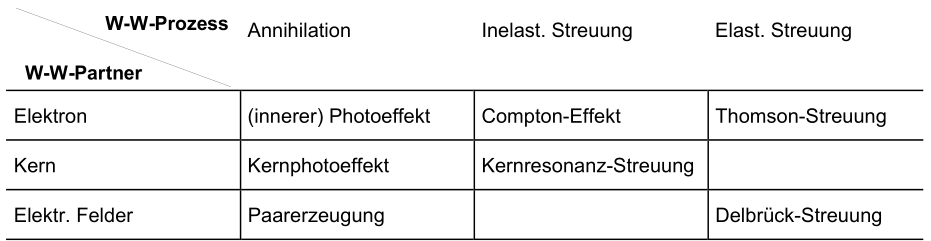
\includegraphics[width=\textwidth]{Bilder/Wechselwirkung.png}
    \caption{Wechselwirkungsprozesse der $\gamma$-Strahlung mit Materie \cite{sample}.}
\end{figure}
Die drei dominierenden Effekte sind hier Photo- und Compton-Effekt und die Paarbildung.

\subsubsection{Photoeffekt}
\label{sec:Photoeffekt}
Trifft das $\gamma$-Quant auf einen Hüllenelektron, so wird das Elektron herausgelöst und das Photon vernichtet.
Es erhält dabei die Energie
\begin{align*}
    E_{\symup{e}} = hf - E_{\symup{B}}.
\end{align*}
Dabei ist $E_{\symup{B}}$ die Bindungsenergie des Elektrons. Damit der Photoeffekt auftritt, muss das Photon
mindestens die Bindungsenergie des Elektrons haben.

\subsubsection{Compton-Effekt}
\label{sec:Compton-Effekt}
Beim Compton-Effekt trifft das Photon auf ein freies Elektron, wie es zum Beispiel bei den leitenden Elektronen
von Metallen zu finden ist. Dabei wird das Photon inelastisch gestreut und gibt einen Teil seiner Energie an das
Elektron ab. Dieser Prozess ist in Abbildung 2 dargestellt.
\begin{figure}
    \centering
    \label{fig:compton}
    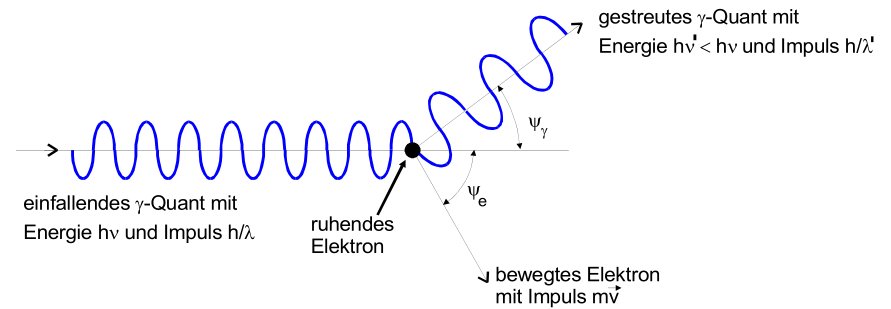
\includegraphics[width=\textwidth]{Bilder/Compton.png}
    \caption{Schematische Darstellung des Comptoneffekts \cite{sample}.}
\end{figure}
Der Wirkungsquerschnitt $\sigma_\text{C}$ wird durch
\begin{equation}
	\sigma_\text{C}=2\pi  r_e^2\left(\frac{1+\epsilon}{\epsilon²}\left(\frac{2(1+\epsilon)}{1+2\epsilon}-\frac{1}{\epsilon}\ln(1+2\epsilon)\right)+\frac{1}{2\epsilon}\ln(1+2\epsilon)-\frac{1+3\epsilon}{(1+2\epsilon)²}\right)
\label{eq:sigma_c}
\end{equation}
mit $\epsilon=\frac{E_{\gamma}}{m_0c²}$ und dem kleinsten Elektronenradius $r_e=\SI{2.82e-15}{\meter}$ beschrieben. 
Daraus folgt dann für den Absorptionskoeffizienten:
\begin{equation}
	\mu_\text{C}=n\sigma_\text{C}(\epsilon)=\frac{Z N_L \rho}{M}\sigma_\text{C}(\epsilon).
\label{eq:mu_c}
\end{equation}

\subsubsection{Paarerzeugung}
\label{sec:Paarerzeugung}
Wenn die Energie des $\gamma$-Quants größer als die doppelte Ruhemasse des Elektrons ist, also
\begin{align*}
    E_{\symup{\gamma}} > 2m_{\symup{0}}c^2 = 1,02\,\unit{\mega\eV}
\end{align*}
gilt, dann kann das Photon durch Erzeugung eines Elektrons und eines Positrons annihiliert werden.\\
\\
In Abbildung 3 ist der Extinsionskoeffizient gegen die Energie aufgetragen und die Anteile von Photo- und
Compton-Effekt und der Paarerzeugung aufgeschlüsselt.
\begin{figure}
    \centering
    \label{fig:Extinsionskoeffizient}
    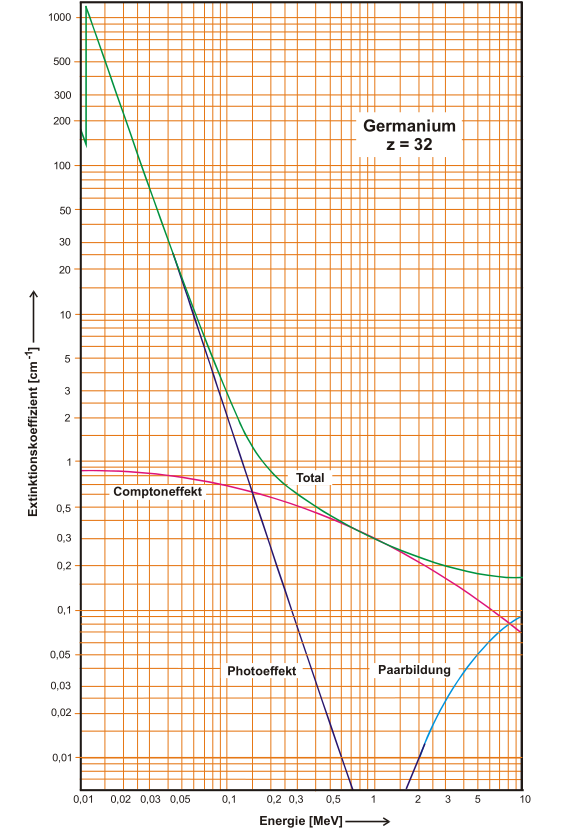
\includegraphics[scale=0.75]{Bilder/Energieabhaengigkeit.png}
    \caption{Energieabhängigkeit des Extinsionskoeffizienten \cite{sample}.}
\end{figure}
Der Photoeffekt ist vorallem bei niedrigen Energien von Relevanz, da er mit der Energie linear abfällt.
Bei mittleren Energien dominiert hauptsächlich der Compton-Effekt bis bei ca. $1\,\unit{\mega\eV}$ die
Paarbildung beginnt und ansteigt.

\subsection{Betastrahlung}
\label{sec:Betastrahlung}
Bei der $\beta$-Strahlung handelt es sich hauptsächlich um Elektronen bei $\beta^{-}$- und Positronen bei
$\beta^{+}$-Strahlung. Diese entsteht, wenn ein Neutron in ein Proton oder ein Proton in ein Neutron umgewandelt
wird. Weiterhin wird dabei noch ein Antineutrino oder eine Neutrino aufgrund der Leptonenzahlerhaltung emmitiert.
\begin{align*}
    n &\rightarrow p + e^{-} + \bar{\nu_{\symup{e}}}\\
    p &\rightarrow n + e^{+} + \nu_{\symup{e}}
\end{align*}
Da die Wechselwirkung eines Neutrinos mit Materie verschwinden gering ist, wird es hier vernachlässigt.\\
\\
Obwohl eine Vielzahl von Prozessen auftritt, wird die Wechselwirkung hauptsächlich nur von den folgenden
drei Prozessen bestimmt.

\subsubsection{Elastische Streuung am Atomkern}
\label{sec:elastischeStreuung}
Die Elektronen werden am Coulomb-Feld des Kerns abgelenkt, so dass ein Intensitätsverlust durch Auffächerung des Strahls
auftritt. Außerdem sorgt das Ablenken dafür, dass die Elektronen länger im Material verweilen und somit eine
höhere Wechselwirkungswahrscheinlichkeit haben. Diese Art von Streuung wird Rutherfordstreuung genannt.

\subsubsection{Inelastische Streuung}
\label{sec:inelastischeStreuung}
Die Elektronen werden im Coulomb-Feld der Kerne beschleunigt und geben somit Bremsstrahlung ab, so dass insgesamt
auch ein Intensitätsverlust festzustellen ist.

\subsubsection{Inelastische Streuung an den Elektronen des Absorbermaterial}
\label{sec:inelastischeStreuungAbsorber}
Die $\beta$-Teilchen treffen auf die Elektronen des Materials und sorgen dort für eine Ionisation bei
der sie Energie abgeben. Da nur ein geringer Teil der Energie abgegeben wird, sind die $\beta$-Teilchen
in der Lage eine Vielzahl dieser Prozesse durchzuführen.\\
\\
Durch die unterschiedlichsten Prozesse, die bei der Absorption von $\beta$-Strahlung auftreten, lässt sich
die Absorptionskurve nicht leicht herleiten. Für geringe Schichtdicken gilt ein Absorptionsgesetz wie in
\autoref{eqn:Absorptionsgesetz}. Nähert sich die Schichtdicke der maximalen Reichweite kommt es nur noch
zur Untergrundstrahlung. In Abbildung 4 ist dieser Zusammnehang dargestellt.
\begin{figure}
    \centering
    \label{fig:Absorptionskurveb}
    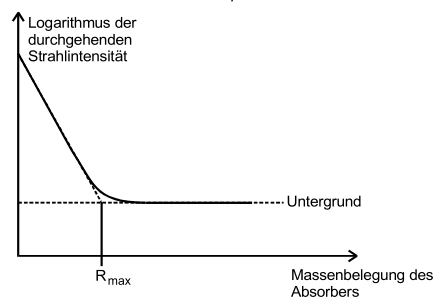
\includegraphics{Bilder/Absorptionskurve.png}
    \caption{Absorptionskurve für einen natürlichen $\beta$-Strahler \cite{sample}.}
\end{figure}
Hierbei ist nicht die Schichtdicke sondern die Massenbelegung $R$ aufgetragen, die durch
\begin{align}
    \label{eqn:Massenbelegung}
    R = \rho D
\end{align}
bestimmt ist. Durch eine lineare Regression in Abbildung 4 lässt sich
dadurch $R_{max}$ bestimmen. Da $R_{max}$ hauptsächlich von den energiereichsten Elektronen abhängt, lässt sich
empirisch auf $E_{\symup{max}}$ schließen, so dass sich
\begin{align}
    \label{eqn:emax}
    E_{\symup{max}} = 1,92 \sqrt{R_{\symup{max}}^2 + 0,22\cdot R_{\symup{max}}} \,\, [\unit{\mega\eV}]
\end{align}
ergibt.